\chapter{Performance profiling at the bytecode level} % for fun and profit
\label{chap:profiling-bytecode}

%% Top-level summary
% Hook
Performance profilers are powerful tools, providing useful information about program control flow and hotspots -- facilitating performance optimisation.
% Argument
However, the feature set and granularity of these tools must match that of the program they are being applied to.
% Link

%% Research gap
% Hook
Existing profilers for Python operate at the function or line level.
% Argument
% cProfile
% scalene
% + 1 other?
% Link

\vspace{1em}
\begin{code}
    \centering
    \begin{minted}[fontsize=\footnotesize]{text}
      214 function calls (207 primitive calls) in 0.002 seconds

Ordered by: cumulative time

ncalls  tottime  percall  cumtime  percall filename:lineno(function)
     1    0.000    0.000    0.002    0.002 {built-in method builtins.exec}
     1    0.000    0.000    0.001    0.001 <string>:1(<module>)
     1    0.000    0.000    0.001    0.001 __init__.py:250(compile)
     1    0.000    0.000    0.001    0.001 __init__.py:289(_compile)
     1    0.000    0.000    0.000    0.000 _compiler.py:759(compile)
     1    0.000    0.000    0.000    0.000 _parser.py:937(parse)
     1    0.000    0.000    0.000    0.000 _compiler.py:598(_code)
     1    0.000    0.000    0.000    0.000 _parser.py:435(_parse_sub)
    \end{minted}
        \caption{Profiling results of \texttt{cProfile.run('re.compile("foo|bar")')} are at the granularity of function calls.}
        \label{listing:cprofile-example}
\end{code}

%% Our tool and its goals
% Hook
Recent developments to CPython's runtime motivate collecting more fine-grained profiling information.
% Argument
For example, the specialising adaptive interpreter rewrites bytecode at runtime into quickened forms, and the baseline \ac{jit} substitutes bytecode for tier two micro-operations -- both yielding performance characteristics which cannot be reasoned about with function or line level instrumentation.
In addition to this, bytecode performance profiling information helps provide a key missing data point when examining the impact of program dynamism.
One reason for this conspicuous absence of bytecode level profilers is the difficulty of measuring their very short execution times, in the order of highest resolution system counter, deeply interleaved within the interpreter's execution loop.
% Link

%% Our tool and its goals
% Hook
To address this gap in the field, we present ByteSight, a novel tool for the performance profiling of CPython bytecode.
% Argument
ByteSight is a tracing profiler which operates on the bytecode level of the Python interpreter. This provides
% ByteSight is implemented natively in Python, using only the standard library. As such, it is both portable and robust
% Link
In this chapter, we discuss the approach and challenges of its implementation, along with providing examples of its use.


\section{Implementation}
\label{sec:profiling-bytecode-implementation}

%% Dynamic python can be used to instrument itself
% Hook
By virtue of the flexibility of its interpreter's implementation, CPython provides a wide variety of opportunities for instrumenting and introspecting running code.
% Argument
One example of this is the standard library function \mintinline{python}{sys.settrace}, which associates dynamic, user-defined callback functions with the dispatch of key virtual machine events. These include function calls, line execution, handling exceptions, and even individual opcodes.
% Link
This callback function receives the event type along with the CPython frame and code objects currently being evaluated by the interpreter, facilitating precise instrumentation of the internal operation of the interpreter.

%% Sketch of approach
% Hook
Our tool captures bytecode level profiling information through a custom callback function which records a sequence of timestamps associated with the traced events.
% Argument
From this set of timestamps, we can calculate the execution duration of each emitted opcode. This constitutes profiling information of a higher granularity than existing Python performance profilers.
Despite its name, we leverage the \mintinline{python}{sys.settrace} function instead of \mintinline{python}{sys.setprofile}. This is because since Python 3.7, \mintinline{python}{sys.settrace} has supported emitting trace events for opcodes, whereas \mintinline{python}{sys.setprofile} only emits events at the function granularity.
% Link

%% Challenges associated with approach
% Hook
This approach presents a number of challenges.
% Argument
% Link
% Requires tight co-design with CPython
To navigate these challenges, we carefully co-design our tracing function with CPython's interpreter loop and tracing infrastructure in mind.


\subsection{CPython internals}
\label{ssec:profiling-bytecode-cpython-internals}

% Focus on Python 3.10, stuff has moved around in more recent versions, but still in legacy_tracing with backwards compatability so all OK. LLTrace is a thing but doesn't give us the timing information we want

%% Interpreter loop, specific to CPython3.10. LLTrace/profile don't give us what we want
% Hook
Due to the short execution duration
% Argument
In this section, we present a view of the CPython3.10's implementation to justify our measurement approach.
% Link

%% Block diagram?

\begin{figure}[H]
    \centering
    \begin{subfigure}[b]{0.65\textwidth}
        \centering
        \begin{minted}[breakanywhere,fontsize=\scriptsize,escapeinside=££]{text}
PyObject* _PyEval_EvalFrameDefault(PyThreadState *tstate, PyFrameObject *f, int throwflag) {
    // ... declarations and initialization of local variables, macros definitions, call depth handling, ...
    // ... code for tracing call event

    for (;;) {
        // NEXTOPARG() macro
        _Py_CODEUNIT word = *next_instr;
        opcode = _Py_OPCODE(word);
        oparg = _Py_OPARG(word);
        next_instr++;

        // ... code for tracing opcode events

        switch (opcode) {
            case TARGET(NOP) {
                FAST_DISPATCH();
            }
            case TARGET(LOAD_FAST) {
                // ... code for loading local variable
            }
            // ... 117 more cases for every possible opcode
        }
    }
    // ... termination
}
        \end{minted}
        \captionsetup{name=Listing}
        \caption{Overview of CPython's evaluation loop implementation \cite{victorskvortsovPythonScenes42020}.}
        \label{listing:cpython-evaluation-overview-code}
    \end{subfigure}
    \hfill
    \begin{subfigure}[b]{0.3\textwidth}
       \centering
       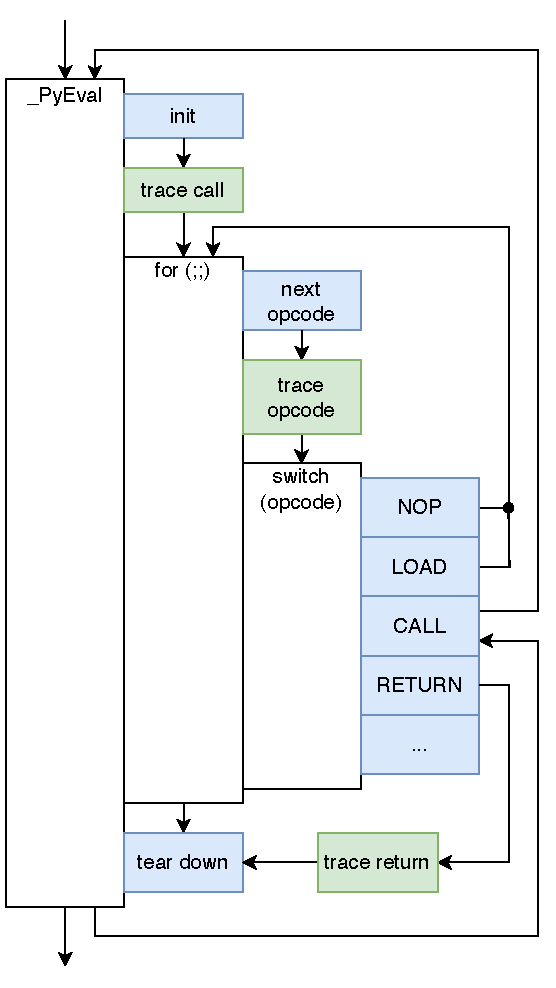
\includegraphics[width=\textwidth]{images/profiling_bytecode/python_eval.drawio.pdf}
    %    \vspace{1em}
       \caption{Block diagram of CPython's evaluation loop implementation.}
       \label{figure:cpython-evaluation-overview-block}
    \end{subfigure}
    \vspace{1em}
    \captionsetup{name=Listing}
    \caption{.}
    \label{figure:cpython-evaluation-overview}
\end{figure}


%% Registering and using a trace function
% Hook
The first step in the tracing process is registering the callback function.
% Argument
To do this, Python users can invoke \mintinline{python}{sys.settrace}, a standard library function binding to the C implementation \texttt{sysmodule.c:sys\_settrace}. This in turn invokes \texttt{ceval.c:\_PyEval\_SetTrace}, which updates two values on of the Python \ac{gil} thread state: \texttt{c\_tracefunc} and \texttt{c\_traceobj}. The former points to a ``trampoline'' function which collects the information required by the callback function, and the latter is a callable python code object for the callback function.
% Link


\subsection{Approach}
\label{ssec:profiling-bytecode-approach}

%% Our approach is...
% Hook
% Argument
% Link

%% Listing of our tracing function

%% This gives us measurements within the CPython runtime
% Hook
This tracing function provides us with a sequence of timestamps for points in the execution stream.
% Argument
From this sequence of timestamps, we need to synthesise the durations of each opcode.
We can reason about this by flattening the block diagram of the evaluation loop (\autoref{figure:cpython-evaluation-overview-block}) and annotating it with the timestamp measurements (\autoref{}).
% Link

%% Figure showing trace events, possibly side-by-side with equations?

%% From these, we can calculate the time taken by each opcode
% Hook
% Argument
% Link


% % TODO: Could interleave this??
% \subsection{Challenges}
% \label{ssec:profiling-bytecode-challenges}

%% Timer granularity + other tricks
% Hook
Beyond the careful co-design of the tracing measurement logic with CPython's implementation, there are a number of confounding effects which must be mitigated to ensure accurate measurement.
% Argument
Firstly, for the profiling information to be useful, the resolution of the most accurate system clock must be sufficient to resolve differences bytecode execution time. On our experimental hardware (\autoref{ssec:experimental-setup}) this was true, having a $1$ns timer able to resolve bytecode taking around $10$ns to execute. However, this is not the case for modern Apple Silicon devices, having only a $40$ns and hence unable to resolve individual bytecode instruction durations. This is a physical limitation on measuring such necessarily fast operations such as bytecode, and as such can only be resolved by selecting appropriate hardware.
Secondly, the CPython language runtime periodically runs housekeeping tasks such as garbage collection, disrupting the flow of bytecode execution and hence adding random noise to our measurements. These can effects can be minimised using techniques from existing performance measurement work such as \texttt{timeit} or \texttt{pyperf}, for example by disabling garbage collection for the duration of profiling.
% Link

%% Warmups + Statistical confidence
% Hook
More generally, we can address noise in our measurements
% Argument
% Link





\section{Example usage}
\label{sec:profiling-bytecode-examples}

%% Simple
% Hook
Having implemented our profiler, we can demonstrate its capabilities on an example workload (Listing \ref{listing:profiler-example}).
% Argument
Each traced event is displayed on its own line, in combination showing the exact sequence of instructions performed by the interpreter when evaluating the function. Function invocations, such as calling \texttt{inner\_function} \circledbase{pairedOneLightBlue}{a}, are indented by their call stack depth for easy readability. In addition to this, bytecode instructions are formatted following the convention of the standard library, but are annotated with their duration in a comment on the right-hand side of the trace \circledbase{pairedTwoDarkBlue}{b}.
% Link


%% Listing function vs profiled bytecode
\begin{figure}[H]
    \centering
    \begin{subfigure}[b]{0.3\textwidth}
       \centering
        \begin{minted}[fontsize=\scriptsize,escapeinside=££]{python}
def inner_function(
    x: int | str | float
) -> None:
    assert x

def example_function() -> None:
    inner_function(1)
    pass
    _x = perf_counter()
        \end{minted}
        \footnotesize\vspace{8em}
        \caption{Python program.}
        \label{listing:profiler-example-python}
    \end{subfigure}
    \hfill
    \begin{subfigure}[b]{0.65\textwidth}
        \centering
        \begin{minted}[fontsize=\scriptsize,escapeinside=££]{text}
// ======= example:6 `example_function` ===-====
// >>> inner_function(1)
7           0   LOAD_GLOBAL          0   (inner_function)   // 15   ns
            2   LOAD_CONST           1   (1)                // 15   ns
            4   CALL_FUNCTION        1   ()                 // 31   ns

    // ======== example:1 `inner_function` ========= £\circledbase{pairedOneLightBlue}{\scriptsize{a}}£
    // >>> assert x
    4           0   LOAD_FAST            0   (x)            // 13   ns
                2   POP_JUMP_IF_TRUE     4   (to 8)         // 13   ns
            >>  8   LOAD_CONST           0   (None)         // 12   ns
                10  RETURN_VALUE             ()             // 31   ns
    // =============================================

            6   POP_TOP                  ()                 // 16   ns
// >>> pass
8           8   NOP                      ()                 // 15   ns £\circledbase{pairedTwoDarkBlue}{\scriptsize{b}}£
// >>> _x = perf_counter()
9           10  LOAD_GLOBAL          1   (perf_counter)     // 15   ns
            12  CALL_FUNCTION        0   ()                 // 17   ns
            14  STORE_FAST           0   (_x)               // 14   ns
            16  LOAD_CONST           0   (None)             // 13   ns
            18  RETURN_VALUE             ()                 // 28   ns
// =============================================
        \end{minted}
        \caption{Profiler output.}
        \label{listing:profiler-example-bytecode}
    \end{subfigure}
    \vspace{1em}
    \captionsetup{name=Listing}
    \caption{Output of the bytecode profiling tool for a simple Python program, showing the sequence of dispatched bytecode and their individual execution times.}
    \label{listing:profiler-example}
\end{figure}


%% Summary/why should I care?
% Hook
% Argument
% Link forward to where it is used in other places
% Link
